% !TeX spellcheck = de_DE
\section{Geschäftsprozesse}
\subsection{Idealtypische Phasen eines Unternehmens}
\begin{multicols}{2}
	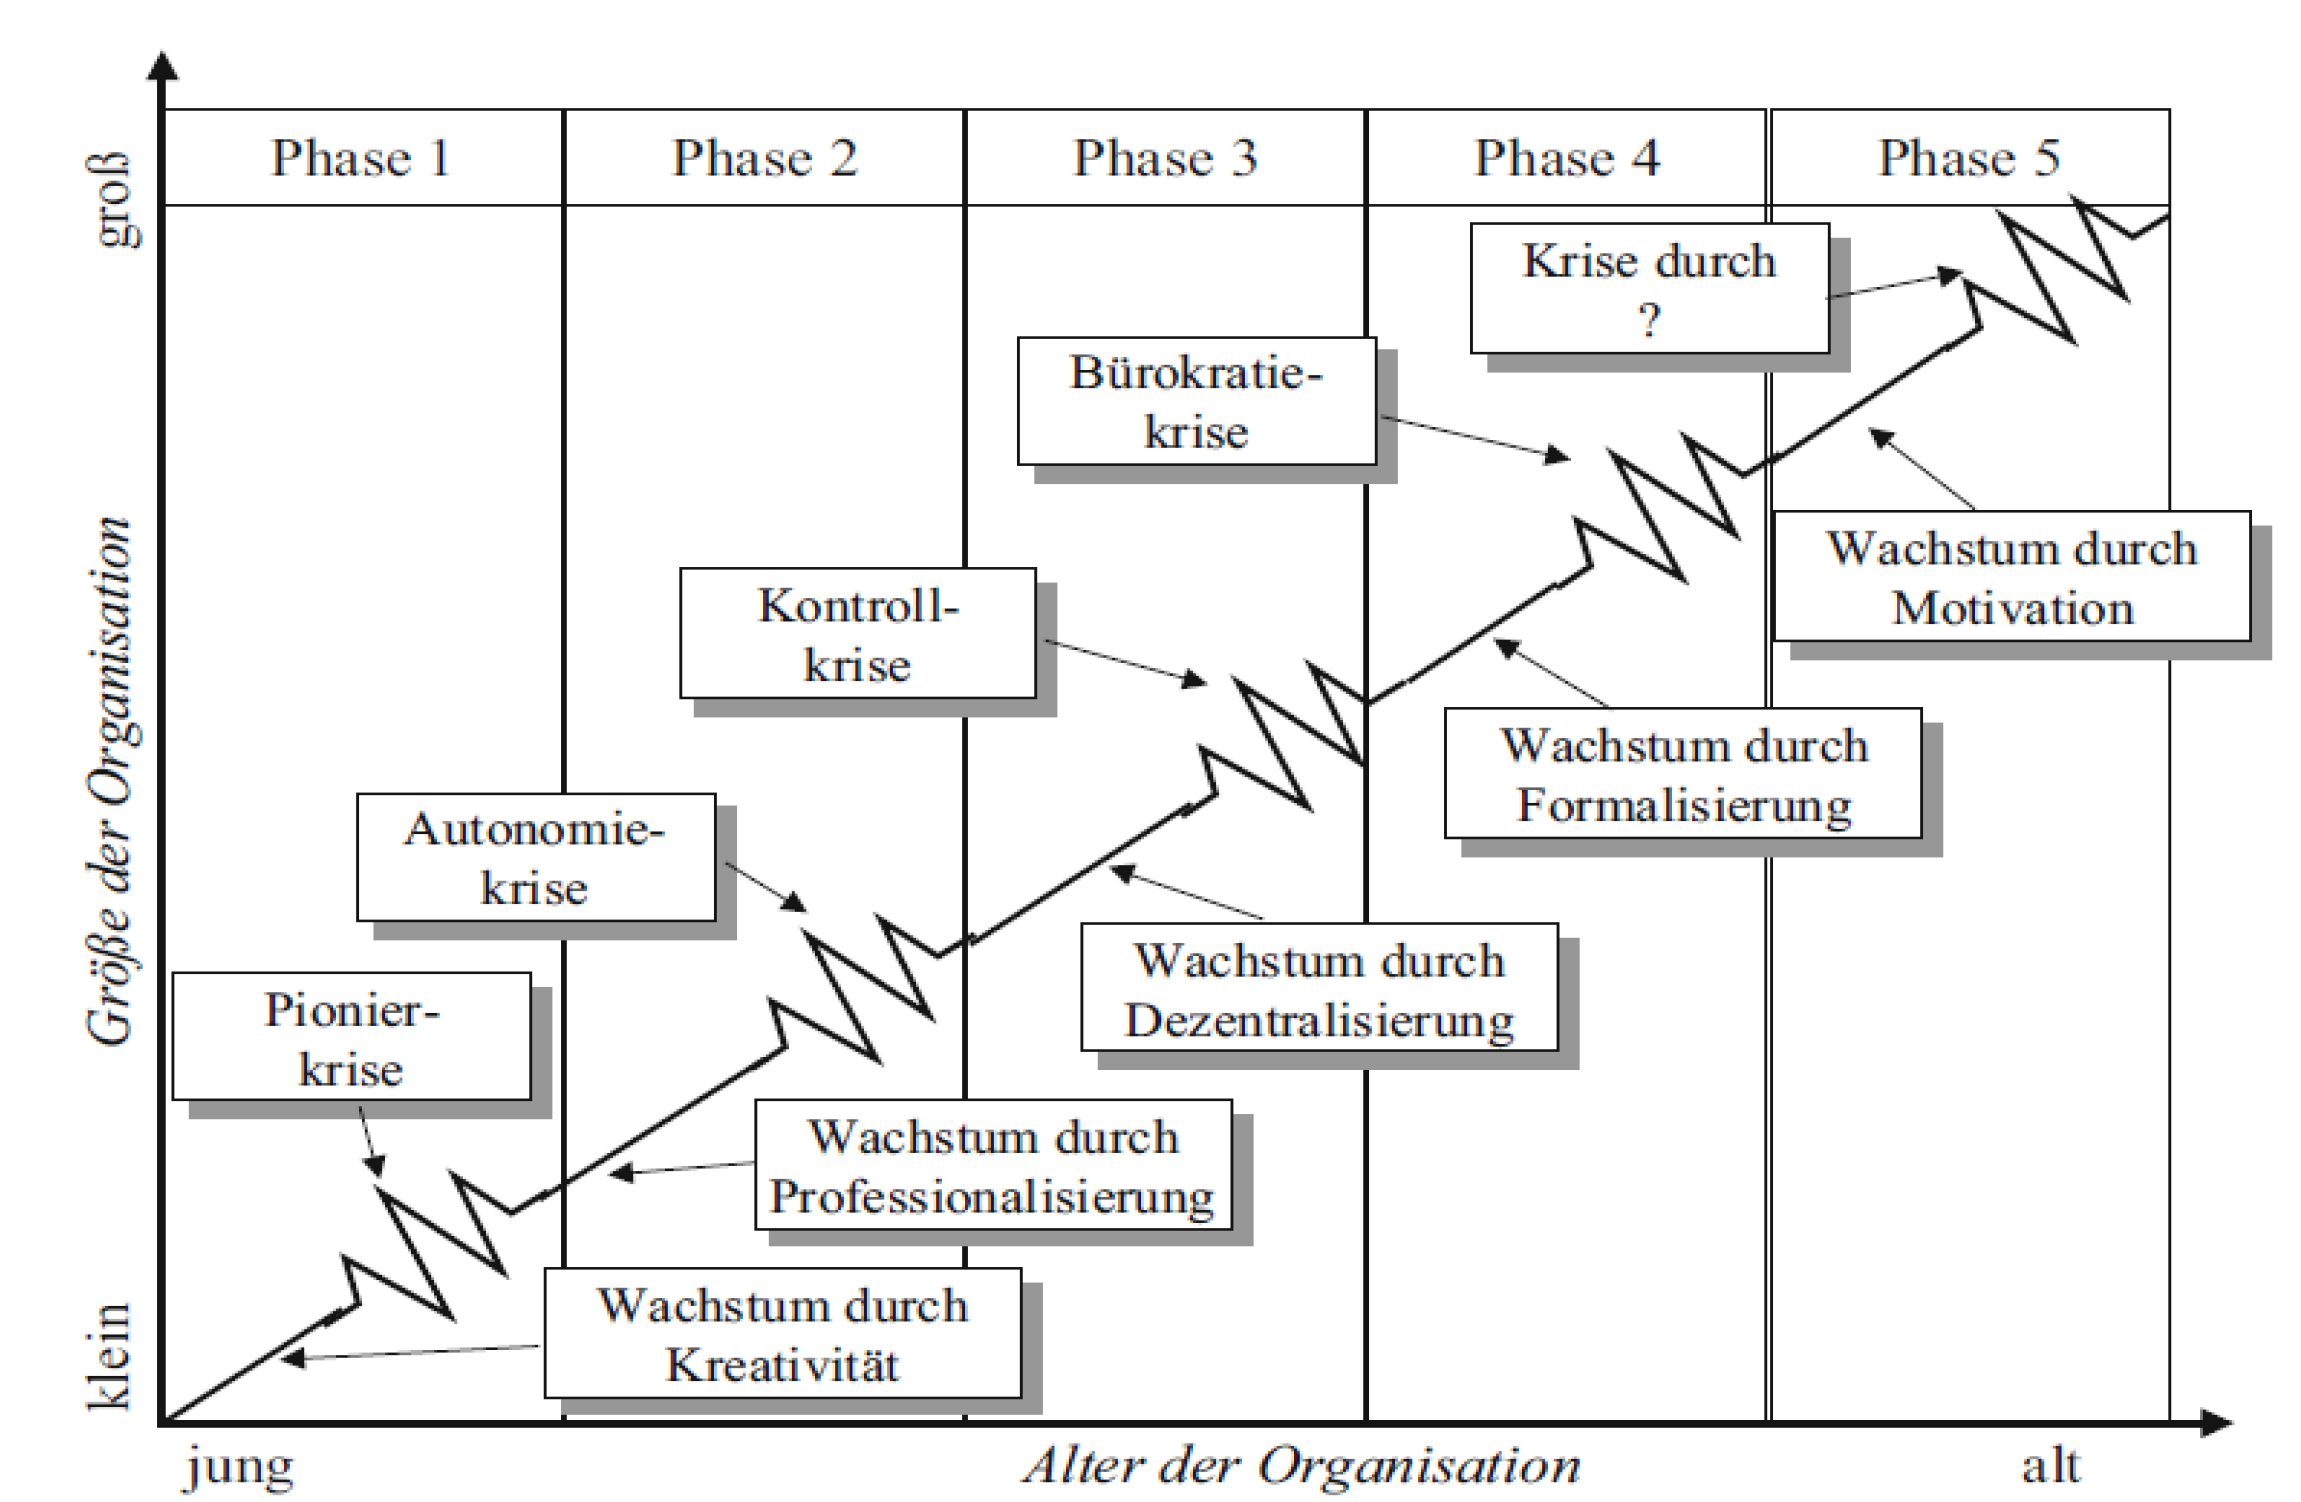
\includegraphics[width=1\linewidth]{images/phasen}
	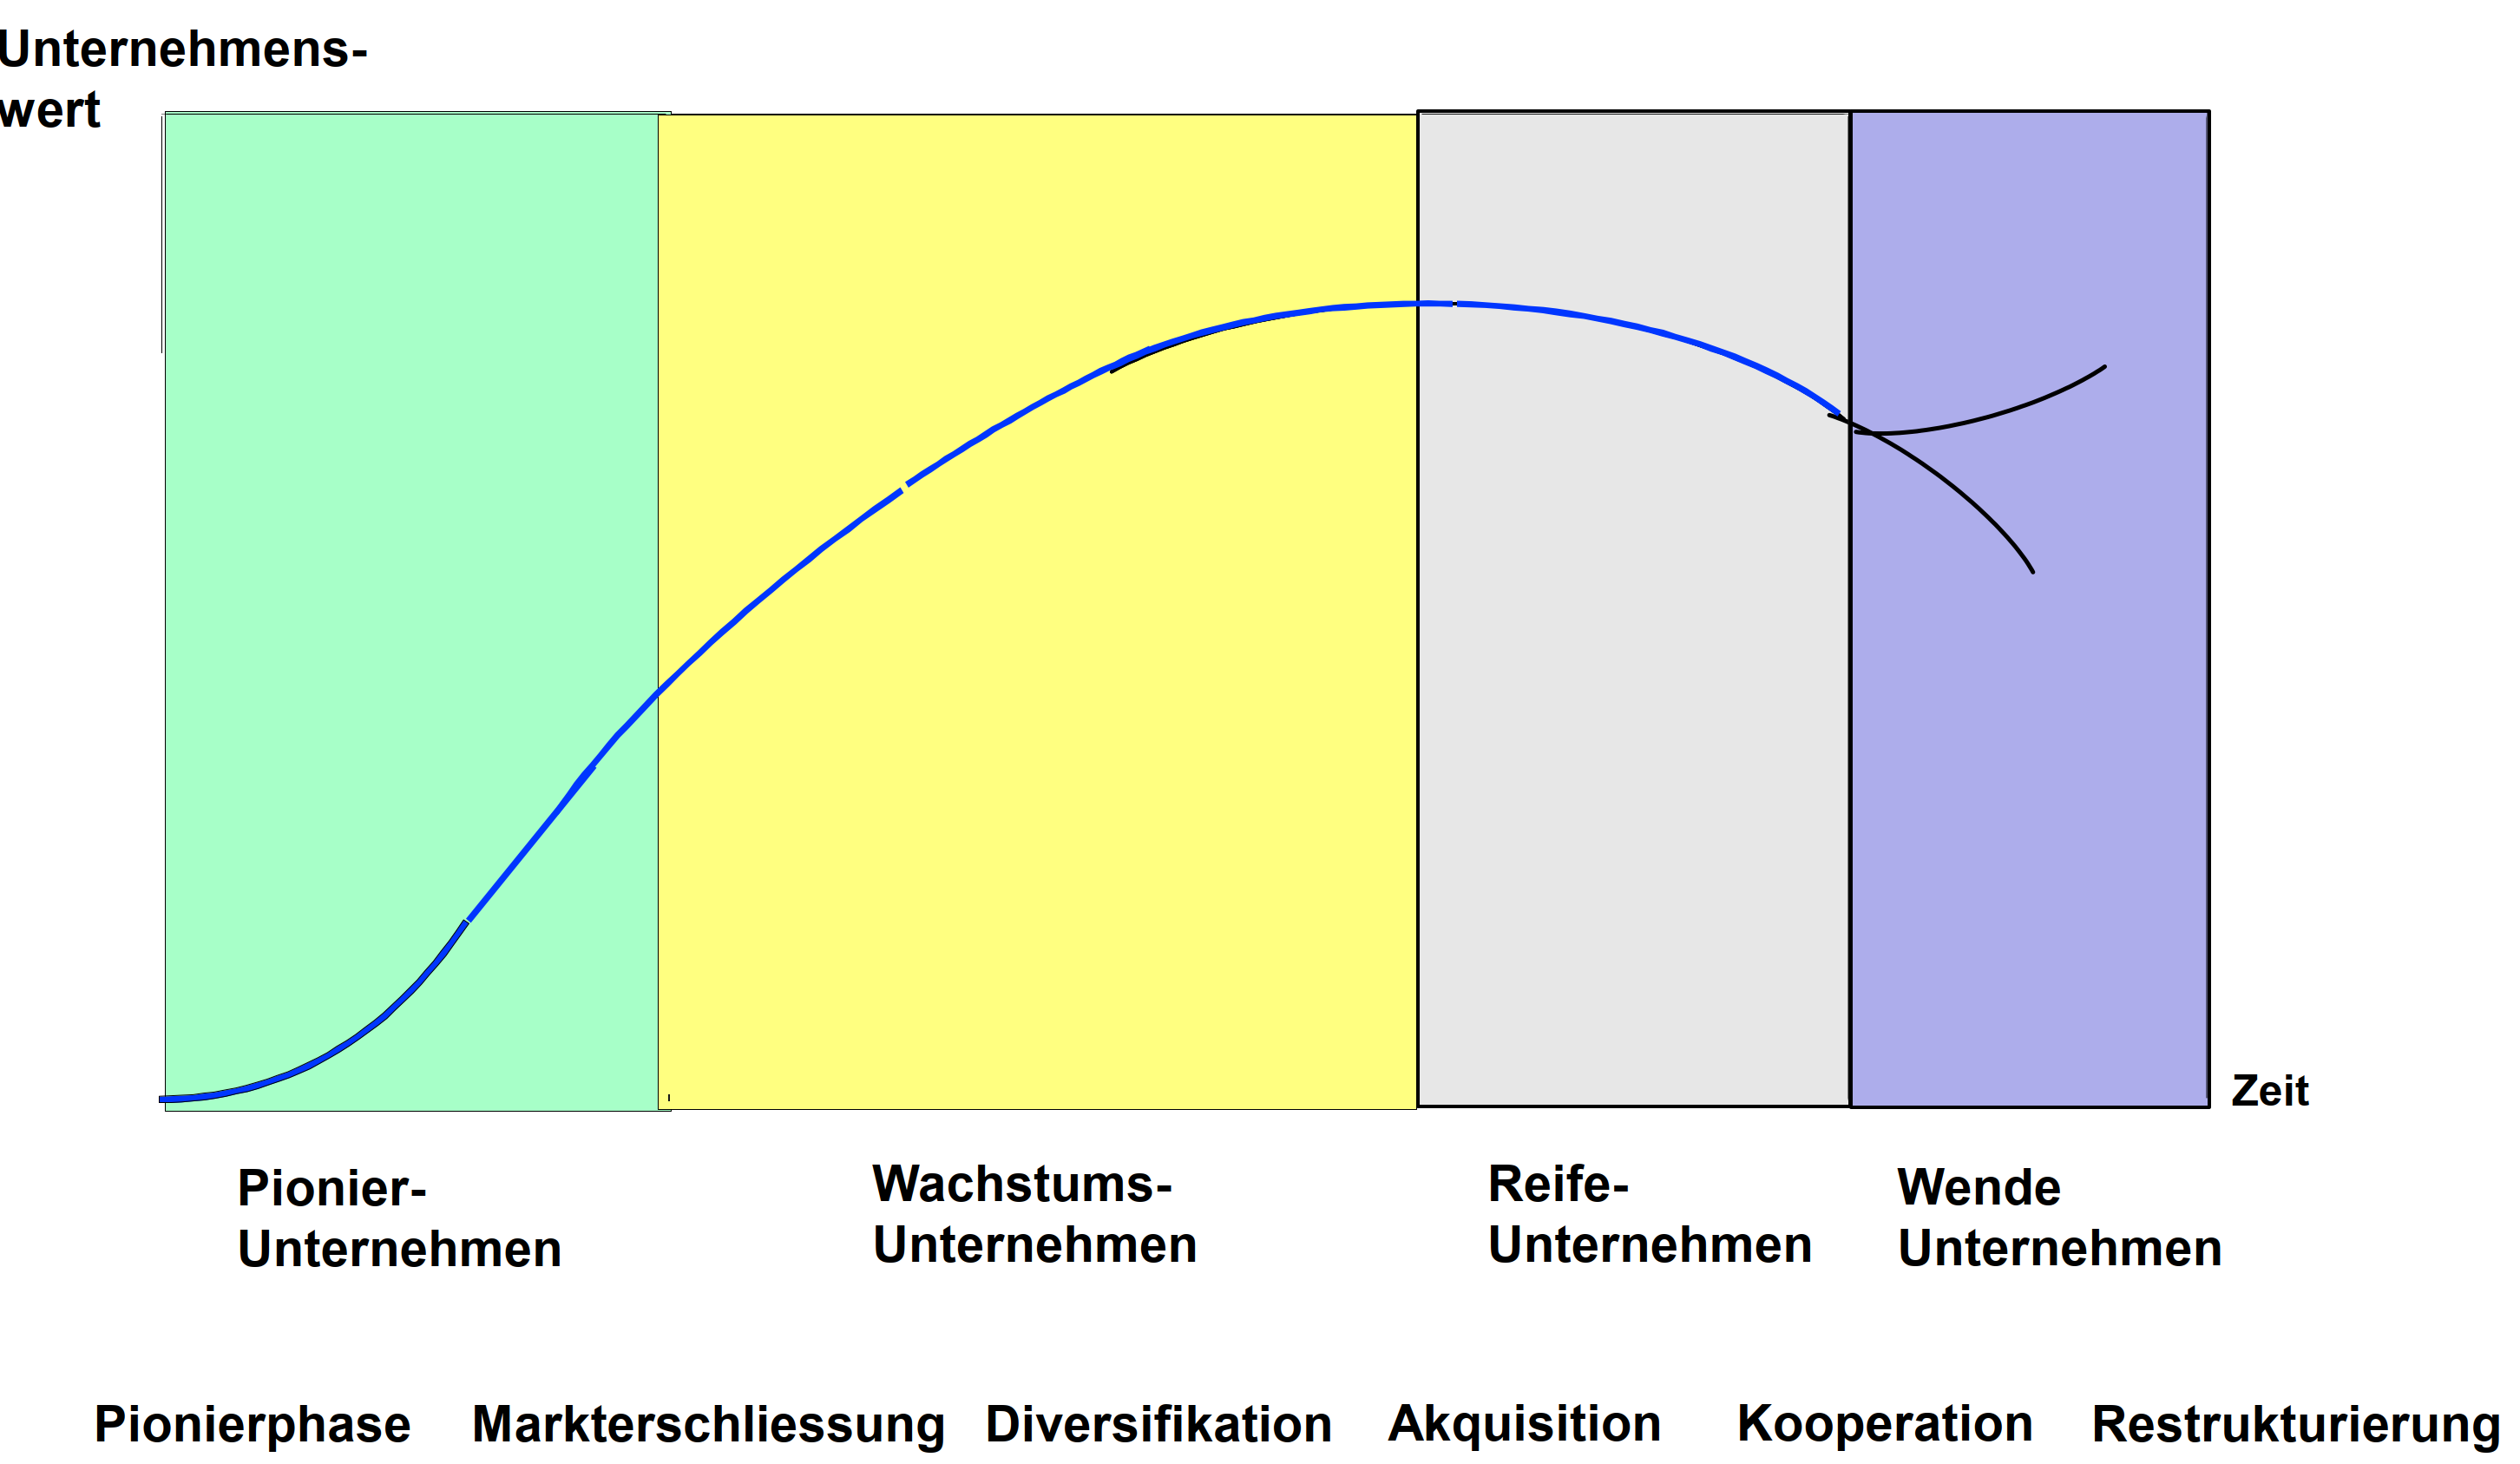
\includegraphics[width=1\linewidth]{images/phasen_2}
\end{multicols}

\subsubsection{Pionierphase}
\begin{itemize}
	\item Idee, technologische Innovation in marktfähiges Produkt oder DL
	\item Wenige Kunden, wenige Beschäftigte
	\item Beherrschung der Produkttechnologie und Produktgestaltung
	\item Probleme des Aufbaus in Griff bekommen
	\item Hohen Finanzbedarf stillen
	\item Allgemeine Aufbruchstimmung
	\item Umsetzung kreativer Ideen
	\item Chaotische Improvisation ohne Regeln und Kontrolle
	\item Keine formalen Strukturen oder Regeln
	\item Koordination „auf Zuruf“ durch persönliche Weisungen
	\item Unstrukturierte, flexible Organisation mit hoher Entwicklungsdynamik
	\item Unternehmensziele = Ziele des Gründers (überragende Stellung)
	\item Hohes Krisenpotenzial (unzureichendes Marktpotenzial, Knappheit finanzielle Mittel, unzureichende betriebswirtschaftliche Professionalität)
\end{itemize}

\subsubsection{Markterschliessung}
\begin{itemize}
	\item Vermittlung des Nutzen des Produkts an breitere Kundenkreise
	\item Unternehmen wächst zu schnell für personelle und materielle Ressourcen-Erweiterung
	\item Gründerunternehmer wird überfordert
	\item Durch erhöhten Kapitalbedarf neue Teilhaber oder Gang an die Börse (IPO)
	\item Veränderung der Eigentümerstruktur und Machtverhältnisse
	\item Professionelles Management übernimmt oberste Unternehmensleitung
	\item Geschäftsprozesse werden standardisiert
	\item Neue Organisationsstrukturen: funktional, da noch homogene Produktstruktur
	\item Damit verbundene Zentralisierung belastet oberste Unternehmensleitung	übermässig mit Entscheidungsaufgaben und Koordinationsproblemen
	\item Geringes Krisenpotenzial, trotzdem: Absatzrückgänge verbunden mit Überkapazitäten und sinkenden Erträgen können existenzbedrohend sein.
\end{itemize}

\subsubsection{Diversifikation}
\begin{itemize}
	\item Entwicklung neuer Geschäftsfelder (aus bestehendem Leistungsprogramm)
	\item Geprägt durch Unternehmergeist und Kreativität
	\item Organisationsstrukturen für neue Aktivitäten: Projektorganisation bzw. Projektmanagement
	\item oder später: Geschäftsbereichsorganisation zur Trennung und autonomen Führung der jeweiligen Produkte und Märkte
	\item Koordination der einzelnen Geschäftsfelder durch oberste Unternehmensleitung
	\item Leistungserbringung hat Professionalität und Effizienz erreicht
	\item Strukturen mit hohem Standardisierungs- und Formalisierungsgrad
	\item Geringes Krisenpotenzial durch Risikostreuung
	\item Nutzung bestehender Erfahrungen in Technologie und Markt
	\item Trotzdem fehlende Erfahrung im Management neuer Produkte (je weiter von ursprünglichen Geschäftsfeldern entfernt)
	\item Unternehmen stösst an Grenzen des Wachstums durch interne Diversifikation
\end{itemize}

\subsubsection{Akquisitionsphase}
\begin{itemize}
	\item Aufbau neuer profitabler Geschäftsfelder durch Übernahme und Integration sowie durch Wachstum von innen (Optimierung)
	\item Entstehung konglomerater Unternehmen durch externe Diversifikation (z.B. unter Holding)
	\item Risiken: Integration neuer Unternehmen und Beibehaltung der alten	Unternehmenskultur
	\item Neue organisatorische Strukturen bei internationalen Akquisitionen: evtl. regionalorientierte statt objektorientierte Geschäftsbereichsorganisation
	\item Überforderung des auf Führung des operativen Geschäfts angelegte Management
	\item Für Integration Vernachlässigung des Stammgeschäfts
\end{itemize}

\subsubsection{Kooperationsphase}
\begin{itemize}
	\item Weg über Akquisition nicht erfolgreich oder an Machbarkeitsgrenzen => Weiterentwicklung über Kooperationen
	\item Franchising, Lizenzvergaben, Joint Ventures, strategische Allianzen
	\item Gewinn von Vertragspartnern für neue Erfolgspotenziale
	\item Kulturell geprägtes, individuelles Verhalten der Partner (hier keine Notwendigkeit der kulturellen Anpassung)
	\item Jeder Wechsel im Management/von Entscheidungsträgern bringt neue Verhaltensweisen
	\item Risiko der Missverständnisse und Misstrauen
	\item Rechtliche und wirtschaftliche Selbständigkeit macht Kooperationsphase zu labilen Form der Unternehmensentwicklung.
\end{itemize}

\subsubsection{Restrukturierungsphase}
Wende-Unternehmen mit zwei möglichen Richtungen:
\begin{itemize}
	\item \textbf{Innere Restrukturierung:} Rückführung in frühere Lebensphase durch Aufgabe der nicht mehr zukunftsträchtigen Geschäftsfelder und Konzentration auf wachstumsträchtige Bereiche, Schrumpfung, Veräusserung von
	Geschäftsfeldern, Aufgabe von Synergien, bis hin zur Integration in anderes Unternehmen
	\item \textbf{Äussere Restrukturierung:} Weg der Schrumpfung und Neuausrichtung nicht mehr möglich; externe Restrukturierungsspezialisten übernehmen das Unternehmen, teilen es auf und veräussern Teile => Untergang des Unternehmens
\end{itemize}

\subsection{Ansoff Matrix}
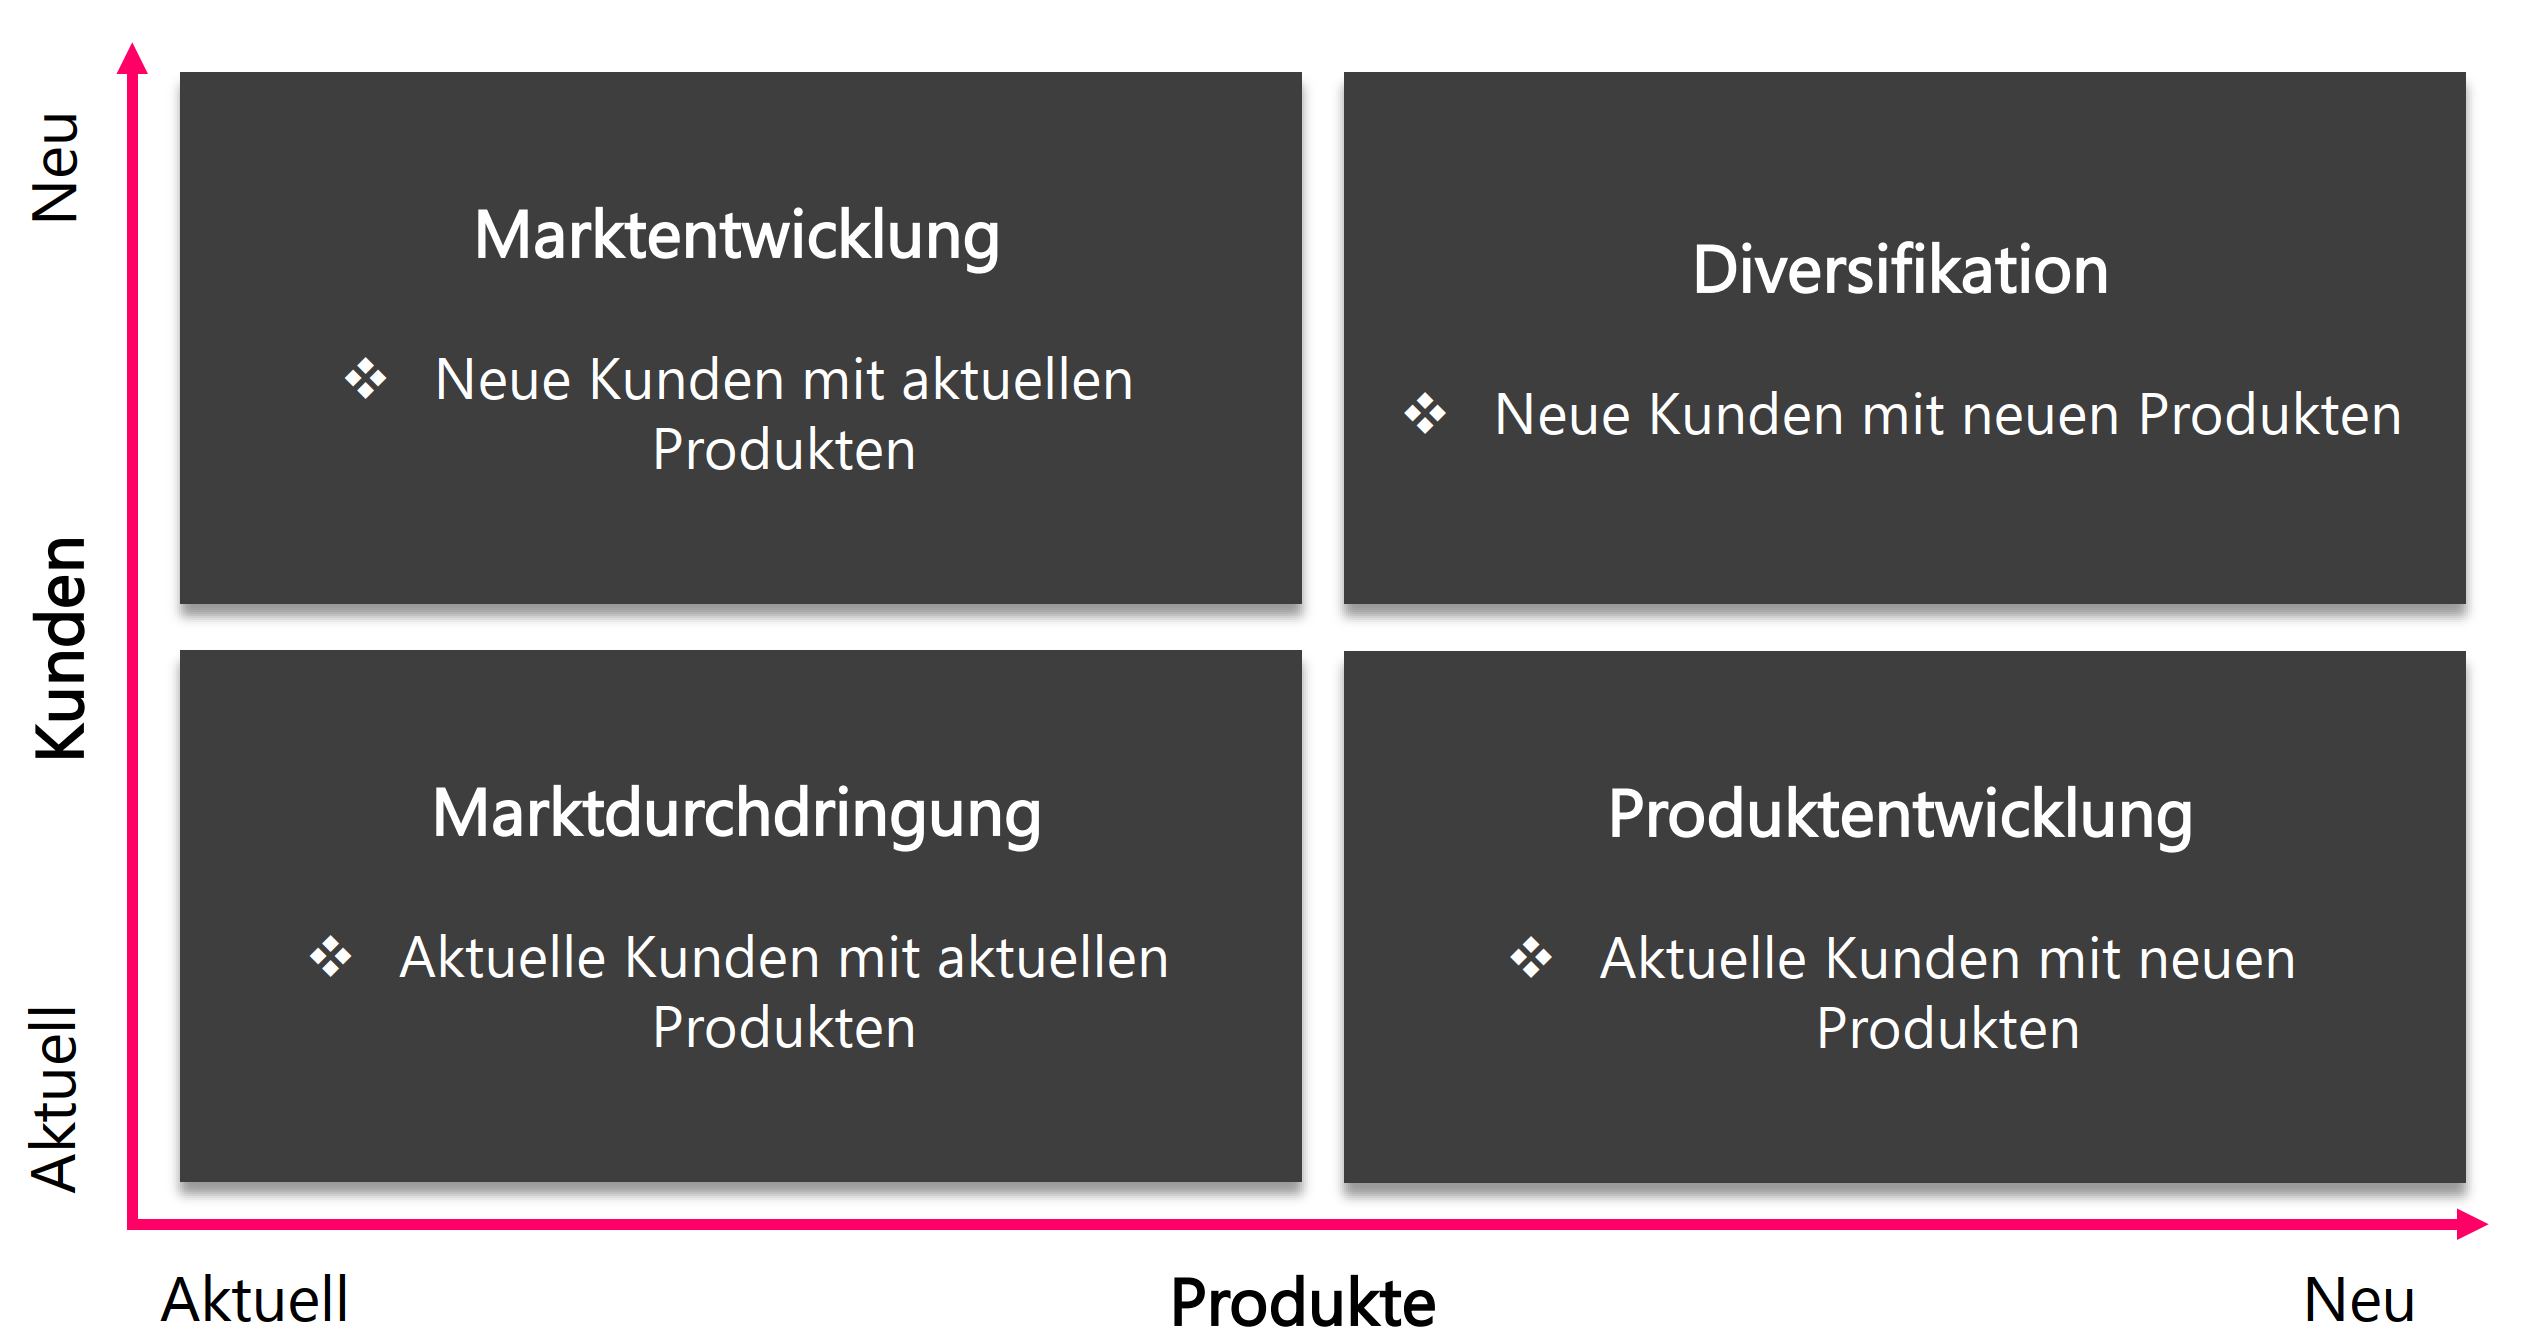
\includegraphics[width=0.5\linewidth]{images/ansoff}